
\chapter{测试与验证}

\section{测试与验证平台介绍}

\subsection{测试硬件平台介绍}
本文所有工作都在龙芯3A-780E开发板上进行,相关硬件平台信息如下表所示\cite{3A-780E}:

\begin{center} \tablecaption{测试硬件平台信息 \label{tab:hardware-platform}} 
\tablefirsthead{
\rowcolor[gray]{0.8}
\multicolumn{1}{c}{\textbf{CPU}} &
\multicolumn{1}{c}{\textbf{内存}} &
\multicolumn{1}{c}{\textbf{GPU}} &
\multicolumn{1}{c}{\textbf{显存}} \\ }
\tablehead{\multicolumn{3}{c}{
\small 表 \ref{tab:hardware-platform} (续) } \\
\rowcolor[gray]{0.8}
\multicolumn{1}{c}{\textbf{CPU}} &
\multicolumn{1}{c}{\textbf{内存}} &
\multicolumn{1}{c}{\textbf{GPU}} &
\multicolumn{1}{c}{\textbf{显存}} \\ }
\tabletail{\bottomrule
\multicolumn{4}{c}{\small 接下页} \\}
\tablelasttail{\bottomrule}

%./svPerfGL -i ../../trisNormsColors-512.nc -w 1280 -h 1024 -2 -r -t 60 -s 3000000
\begin{supertabular}{p{5.5cm}<{\centering}p{2.cm}<{\centering}p{5.5cm}<{\centering}p{2.cm}<{\centering}}
	longson 3A, 800M Hz& &  RS780E, 500M Hz& \\
	4 GS464 Core&  & Radeon HD 3200 & \\
	64KB L1 Data Cache/Core&  2GB&  40 Unified Pipeline& 128MB\\
	64KB L1 Instruction Cache/Core&  &  55 nm& \\
	4MB L2 Cache &  &  & \\
\end{supertabular}
\end{center}

相关软件平台如下表所示:

\begin{center} \tablecaption{测试软件平台信息 \label{tab:software-platform}} 
\tablefirsthead{
\rowcolor[gray]{0.8}
\multicolumn{1}{c}{\textbf{操作系统}} &
\multicolumn{1}{c}{\textbf{内核版本}} &
\multicolumn{1}{c}{\textbf{Mesa3D库版本}} &
\multicolumn{1}{c}{\textbf{libdrm库版本}} &
\multicolumn{1}{c}{\textbf{glibc库版本}} \\ }
\tablehead{\multicolumn{3}{c}{
\small 表 \ref{tab:software-platform} (续) } \\
\rowcolor[gray]{0.8}
\multicolumn{1}{c}{\textbf{操作系统}} &
\multicolumn{1}{c}{\textbf{内核版本}} &
\multicolumn{1}{c}{\textbf{Mesa3D库版本}} &
\multicolumn{1}{c}{\textbf{libdrm库版本}} &
\multicolumn{1}{c}{\textbf{glibc库版本}} \\ }
\tabletail{\bottomrule
\multicolumn{5}{c}{\small 接下页} \\}
\tablelasttail{\bottomrule}

%./svPerfGL -i ../../trisNormsColors-512.nc -w 1280 -h 1024 -2 -r -t 60 -s 3000000
\begin{supertabular}{p{3.cm}<{\centering}p{3.cm}<{\centering}p{3.cm}<{\centering}p{3.cm}<{\centering}p{3.cm}<{\centering}}
	Fedora 13& 2.6.32 mips64&  10.1.6& 2.4.50& 2.12.2\\
\end{supertabular}
\end{center}

\subsection{svPerfGL测试集介绍}

svPerfGL是一个OpenGL的测试基准。它主要用来测试科学可视化程序的真实性能,这些程序拥有很大的输入负载和OpenGL状态变化,它们以大量的存储格式为netCDF的大量三角形信息作为输入数据,这些三角形都被绘制在同一帧上,然后在用户指定的时间内不断的渲染,统计最后的渲染效率即每秒多少帧(frames/sec),最后将这些性能数据统计出来输出。

svPerfGL主要测试项如下表所示:

\begin{center} \tablecaption{svPerfGL测试项 \label{tab:svPerfGL-introduce}} 
\tablefirsthead{
\rowcolor[gray]{0.8}
\multicolumn{1}{c}{\textbf{测试项}} &
\multicolumn{1}{c}{\textbf{执行参数}} &
\multicolumn{1}{c}{\textbf{说明}} \\ }
\tablehead{\multicolumn{3}{c}{
\small 表 \ref{tab:svPerfGL-introduce} (续) } \\
\rowcolor[gray]{0.8}
\multicolumn{1}{c}{\textbf{测试项}} &
\multicolumn{1}{c}{\textbf{执行参数}} &
\multicolumn{1}{c}{\textbf{说明}} \\ }
\tabletail{\bottomrule
\multicolumn{3}{c}{\small 接下页} \\}
\tablelasttail{\bottomrule}

\begin{supertabular}{p{4.cm}<{\centering}p{2.cm}<{\centering}p{9.cm}<{\centering}}
	立即模式 & & 传统的立即模式绘制,即glBegin()...glEnd()\\
    显示列表模式 & -r & 传统的显示列表模式,即显示列表里面的数据为glVertex() \\
	顶点数组模式 & -v & 例如glDrawArrays()等 \\
	顶点显示列表模式 & -v -r & 显示列表里面数据采用顶点模式收集 \\
\end{supertabular}
\end{center}


\section{CPU与GPU负载平衡优化测试}
为了验证CPU与GPU负载平衡优化效果,在前面所述平台背景下,运行svPerfGL显示列表测试项,在60秒的测试时间内不同数据规模下优化前后测试结果如下表所示:

\begin{center} \tablecaption{svPerfGL显示列表测试项 \label{tab:svPerfGL-dsp}} 
\tablefirsthead{
\rowcolor[gray]{0.8}
\multicolumn{1}{c}{\textbf{输入数据(三角形个数)}} &
\multicolumn{1}{c}{\textbf{优化前性能(frames/s)}} &
\multicolumn{1}{c}{\textbf{优化后性能(frames/s)}} &
\multicolumn{1}{c}{\textbf{提升百分比}} \\ }
\tablehead{\multicolumn{3}{c}{
\small 表 \ref{tab:svPerfGL-dsp} (续) } \\
\rowcolor[gray]{0.8}
\multicolumn{1}{c}{\textbf{输入数据(三角形个数)}} &
\multicolumn{1}{c}{\textbf{优化前性能(frames/s)}} &
\multicolumn{1}{c}{\textbf{优化后性能(frames/s)}} &
\multicolumn{1}{c}{\textbf{提升百分比}} \\ }
\tabletail{\bottomrule
\multicolumn{4}{c}{\small 接下页} \\}
\tablelasttail{\bottomrule}

%./svPerfGL -i ../../trisNormsColors-512.nc -w 1280 -h 1024 -2 -r -t 60 -s 3000000
\begin{supertabular}{p{4.cm}<{\centering}p{4.cm}<{\centering}p{4.cm}<{\centering}p{3.cm}<{\centering}}
	1024& 37.72& 37.85&	0.3$\%$	\\
	4096& 36.87& 36.90&	0.1$\%$	\\
	16384& 30.42& 34.02& 11.8$\%$	\\
	65536& 24.81& 25.79& 4.0$\%$	\\
	262144& 11.31& 12.98& 14.8$\%$	\\
    1048576& 2.20& 3.01& 36.8$\%$	\\
\end{supertabular}
\end{center}

为了更直观的显示优化的成果,将上表\ref{tab:svPerfGL-dsp}的数据绘制成直方图如下:

\begin{figure}[H] 
  \centering
  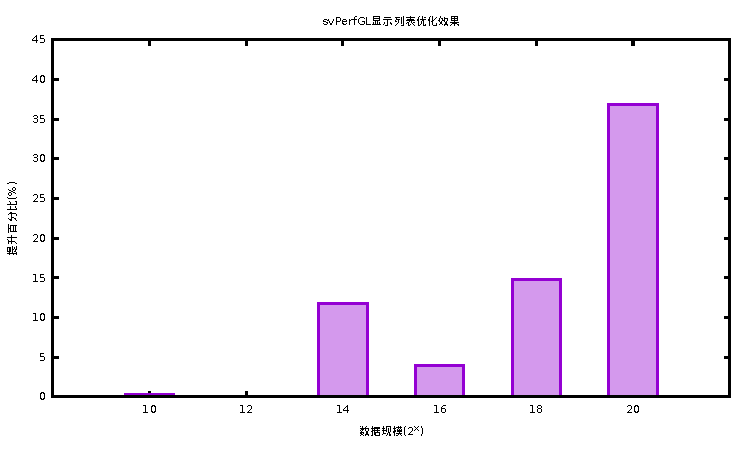
\includegraphics[width=14cm,height=10cm]{figures/gnuplot/result/dsp.eps}
  \caption{Mesa3D图形库显示列表模式优化效果}
  \label{fig:svPerfGL-dsp}
\end{figure}

从图上可以看到在小数据规模小优化效果不明显,这很好理解,因为小数据规模下本身所需缓存数目较少,CPU负载较低。所以负载均衡的优化方法无法发挥作用,当数据规模增大时,优化效果明显增加,在输入数据百万级别时候能达到百分之三十多的性能提升。

\section{Mesa3D的内存到显存的数据传输的优化测试}

为了验证内存到显存的数据传输的优化效果,在前面所述平台背景下,运行svPerfGL顶点数组模式测试项,在60秒的测试时间内不同数据规模下优化前后测试结果如下表所示:

\begin{center} \tablecaption{svPerfGL顶点数组测试项 \label{tab:svPerfGL-vbo}} 
\tablefirsthead{
\rowcolor[gray]{0.8}
\multicolumn{1}{c}{\textbf{输入数据(三角形个数)}} &
\multicolumn{1}{c}{\textbf{优化前性能(frames/s)}} &
\multicolumn{1}{c}{\textbf{优化后性能(frames/s)}} &
\multicolumn{1}{c}{\textbf{提升百分比}} \\ }
\tablehead{\multicolumn{3}{c}{
\small 表 \ref{tab:svPerfGL-vbo} (续) } \\
\rowcolor[gray]{0.8}
\multicolumn{1}{c}{\textbf{输入数据(三角形个数)}} &
\multicolumn{1}{c}{\textbf{优化前性能(frames/s)}} &
\multicolumn{1}{c}{\textbf{优化后性能(frames/s)}} &
\multicolumn{1}{c}{\textbf{提升百分比}} \\ }
\tabletail{\bottomrule
\multicolumn{4}{c}{\small 接下页} \\}
\tablelasttail{\bottomrule}

%./svPerfGL -i ../../trisNormsColors-512.nc -w 1280 -h 1024 -2 -v -t 60 -s 3000000
\begin{supertabular}{p{4.cm}<{\centering}p{4.cm}<{\centering}p{4.cm}<{\centering}p{3.cm}<{\centering}}
	1024& 37.15& 37.83&	\\
	4096& 23.01& 37.29&	\\
	16384& 3.40& 35.63&	\\
	65536& 1.80& 19.77&	\\
	262144& 0.50& 2.40&	\\
\end{supertabular}
\end{center}

为了更直观的显示优化的成果,将上表\ref{tab:svPerfGL-vbo}的数据绘制成直方图如下:

\begin{figure}[H] 
  \centering
  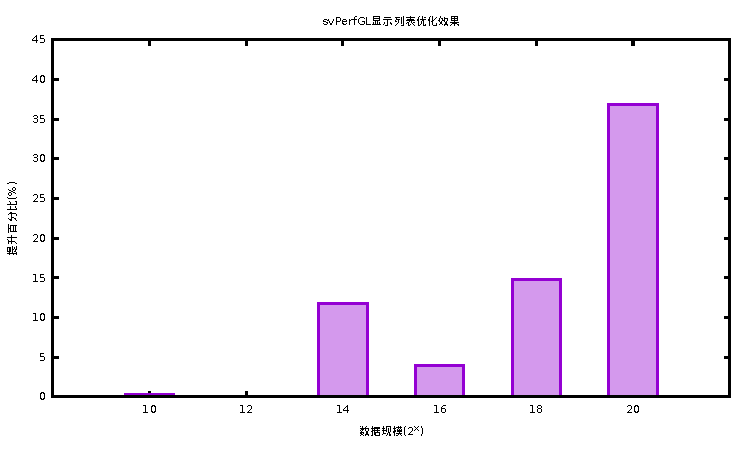
\includegraphics[width=14cm,height=10cm]{figures/gnuplot/result/dsp.eps}
  \caption{Mesa3D图形库显示列表模式优化效果}
  \label{fig:svPerfGL-dsp}
\end{figure}

从上图可以看到XXX

\section{Mesa3D的CPU端优化测试}

为了验证CPU端优化的效果,在前面所述平台背景下,运行svPerfGL立即模式测试项,在60秒的测试时间内不同数据规模下优化前后测试结果如下表所示:

\begin{center} \tablecaption{svPerfGL顶点数组测试项 \label{tab:svPerfGL-imm}} 
\tablefirsthead{
\rowcolor[gray]{0.8}
\multicolumn{1}{c}{\textbf{输入数据(三角形个数)}} &
\multicolumn{1}{c}{\textbf{优化前性能(frames/s)}} &
\multicolumn{1}{c}{\textbf{优化后性能(frames/s)}} &
\multicolumn{1}{c}{\textbf{提升百分比}} \\ }
\tablehead{\multicolumn{3}{c}{
\small 表 \ref{tab:svPerfGL-imm} (续) } \\
\rowcolor[gray]{0.8}
\multicolumn{1}{c}{\textbf{输入数据(三角形个数)}} &
\multicolumn{1}{c}{\textbf{优化前性能(frames/s)}} &
\multicolumn{1}{c}{\textbf{优化后性能(frames/s)}} &
\multicolumn{1}{c}{\textbf{提升百分比}} \\ }
\tabletail{\bottomrule
\multicolumn{4}{c}{\small 接下页} \\}
\tablelasttail{\bottomrule}

%./svPerfGL -i ../../trisNormsColors-512.nc -w 1280 -h 1024 -2 -t 60 -s 3000000
\begin{supertabular}{p{4.cm}<{\centering}p{4.cm}<{\centering}p{4.cm}<{\centering}p{3.cm}<{\centering}}
	1024& & &	\\
	4096& & &	\\
	16384& & &	\\
	65536& & &	\\
	262144& & &	\\
    1048576& & & \\
\end{supertabular}
\end{center}

为了更直观的显示优化的成果,将上表\ref{tab:svPerfGL-imm}的数据绘制成直方图如下:

\begin{figure}[H] 
  \centering
  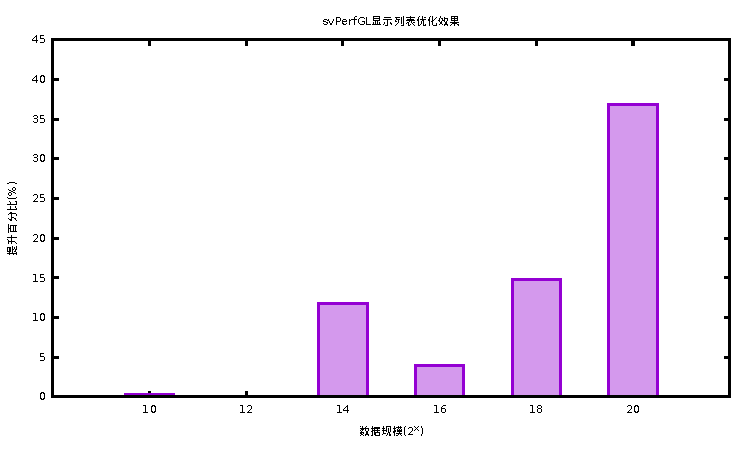
\includegraphics[width=14cm,height=10cm]{figures/gnuplot/result/dsp.eps}
  \caption{Mesa3D图形库显示列表模式优化效果}
  \label{fig:svPerfGL-dsp}
\end{figure}

从上图可以看到XXX

\section{本章小结}

本章显示介绍了实验的平台环境,包括硬件环境和软件配置,并且介绍了用来测试优化效果的svPerfGL测试集。然分别对第三章提出的三个优化方法分别测试和统计优化效果,可以看到三个优化方法虽然适用场景各不相同,但是在对应场景上都有一定的性能提升,特别是显示列表场景中有着很大的提升。总体来说实验效果符合预期,达到优化效果。
